% !TeX root = ../libro.tex
% !TeX encoding = utf8
\chapter{Modules for Experiments in Stellar Astrophysics - MESA}\label{ch:cuarto-capitulo}
\section{Introducción}
Para la realización de este tesis doctoral nos hemos apoyado en la herramienta de evolución estelar \textit{Modules for Experiments in Stellar Astrophysics} (MESA). Este simulador incorpora módulos que se actualizan de manera periódica en base a los avances derivados de los trabajos más novedosos sobre ecuaciones de estado, opacidad, velocidades de reacción nuclear, datos de difusión de elementos y condiciones de límite atmosférico. Es una herramienta muy útil para poder contrastar mediciones obtenidas con los resultados arrojados por un determinado modelo, o para hacer predicciones a partir de modelos y contrastar los resultados que obtenemos de estos con las mediciones disponibles en otros trabajos de investigación.\par

En el caso particular de esta tesis doctoral estamos interesados en estudiar los mecanismos que intervienen en la destrucción de Li en estrellas similares a nuestro Sol, y particularmente en ella. Como hemos comentado a día de hoy no existe una opinión unánime en la comunidad científica, más allá de que los modelos de evolución estelar no producen resultados coherentes con las observaciones, de qué procesos gobiernan el proceso de agotamiento del Li estelar y de cuándo se ponen en marcha o se detienen. Existen diversos planteamientos de procesos que intentan dar una respuesta a este enigma. En este trabajo nos vamos a centrar en cómo influyen en modelos de estrellas de tipo solar, con 1.0 $\msun$ y con una metalicidad (Z) similar al Sol, los efectos de la rotación y de la pérdida de momento angular causada por la presencia de campos magnéticos que inducen un efecto de frenado magnético. Estos campos magnéticos tendrán, en una primera aproximación, una intensidad fija a lo largo de toda la evolución temporal del modelo. Posteriormente se extenderá el modelo para simular campos magnéticos de intensidad variable. Adicionalmente, los modelos simulados se basan en la teoría de la longitud de mezcla para modelar la convección estelar. Este formalismo depende del parámetro libre longitud de mezcla ($\amlt$), parámetro que mayoritariamente tiene un valor preestablecido y fijo durante toda la simulación. En nuestro trabajo, realizaremos simulaciones manteniendo estable el valor de $\amlt$ pero también introduciremos la posibilidad de hacerlo evolucionar temporalmente en base a otros parámetros estelares.\par

En estas circunstancias, nos encontramos en que el primer problema a solventar es el de cómo incorporar estas extensiones al simulador MESA, al mismo tiempo que se respeta su estructura modular y, sobre todo, sin provocar efectos indeseables en el resto de parámetros de la simulación. Para dar solución a este punto tenemos que basarnos en los planteamientos teóricos documentados en el Capítulo \ref{ch:tercer-capitulo} e implementarlos, en forma de rutinas en código Fortran, que puedan ser utilizadas en conjunto con el resto de módulos de MESA.\par

Por otra parte, se hace también necesario el comprender los diferentes parámetros y procesos que MESA utiliza a la hora de calcular las abundancias de los diferentes elementos que podemos encontrar en una estrella a lo largo de su evolución, tanto en su interior como en su atmósfera. Por tanto, aquí tenemos otra área de estudio que pasa por conocer las diferentes capacidades ya disponibles en el simulador que tengan impacto sobre el agotamiento del Li, entender cuándo pasan a ser relevantes en el proceso evolutivo de la estrella, cuáles son los parámetros que gobiernan su funcionamiento, las relaciones que guardan entre ellos y, por último, qué valores son los más recomendables para dar soporte al escenario de simulación que acabamos de plantear.\par

Una vez tengamos la parametrización adecuada para nuestro planteamiento teórico, pasaremos a simular de manera sistemática, haciendo uso de nuestras nuevas rutinas, un conjunto de modelos con diferentes valores para los parámetros relevantes de nuestros modelos: velocidad angular, intensidad del campo magnético y valor de $\amlt$. Los resultados de abundancia de Li que obtengamos en cada uno de los escenarios planteados los enfrentaremos con los que arroja MESA sin hacer uso de nuestra rutina. Esta comparación de resultados nos deberá de dar un primer indicio de si nuestro planteamiento realmente tiene algún efecto notable sobre la abundancia Li detectado en la superficie estelar. Finalmente, en base a los resultados obtenidos, analizaremos las consecuencias que nuestras rutinas han tenido sobre ellos y presentaremos una serie de conclusiones de por qué obtenemos estos datos y cómo se interpretan los mismos en base a los estudios teóricos y observaciones obtenidas por otras líneas de investigación.\par

\subsection{El proyecto MESA}
Como indica su contribuidor y desarrollador principal \author{QUEPONERAQUÍ??} \cite[xxxxxx]{Pasetto2014} (Paxton, et al., 2011, 2013, 2015) MESA es un conjunto de librerías de código abierto, robustas y eficientes escritas en el lenguaje de programación Fortran 95 que es susceptible de ser utilizado en una amplia gama de aplicaciones en astrofísica estelar computacional. Está categorizado dentro de los denominados códigos de evolución estelar unidimensional (1-D) y combina un gran número de módulos numéricos y físicos que le permiten simular una amplia gama de escenarios de evolución estelar, que van desde los que incluyen estrellas de muy baja masa hasta lo que caracterizan estrellas masivas, además de tener en cuenta fases avanzadas de evolución, como el flash del helio, pulsos térmicos o la rama asintótica gigante (AGB). Utiliza un modelo de malla o zonas adaptables, que representa las diferentes capas y celdas en las que se estructura el modelo estelar, y emplea sofisticados controles de evolución temporal.\par

MESA se caracteriza por resolver las ecuaciones de estructura y composición de forma simultánea. Incluye módulos con el último “estado del arte” capaces de resolver las ecuaciones de estado, opacidad, velocidades de reacción nuclear, difusión de elementos y condiciones de límite atmosférico necesarias para realizar la evolución estelar. Cada módulo está construido a partir de una biblioteca desarrollada en Fortran 95 y diseñada de forma modular, diferenciando entre una interfaz pública destinada a ser utilizada por otros módulos y una parte privada donde se implementa la lógica necesaria que permanece inaccesible al resto de módulos. Esta buena práctica permite desarrollar nuevos módulos o revisar los existentes de manera independiente.\par

Por un lado, MESA aborda la física estelar, su estructura y su evolución con métodos numéricos modernos y sofisticados. Por otro, utiliza una física actualizada que le confiere una amplia gama de aplicaciones en diferentes escenarios. Los métodos numéricos y computacionales empleados por MESA le permiten evolucionar de manera consistentemente a través de fases exigentes planteadas por los modelos estelares.\par

MESA se basa en el principio de código abierto: cualquiera puede descargar el código fuente en el que se basa, compilarlo y ejecutarlo para sus propias necesidades de investigación, además de poder ampliar su funcionalidad, como se mostrará a continuación en este trabajo. El propósito de ser distribuido como código abierto es el de involucrar y llegar al mayor número de miembros de la comunidad astrofísica para que hagan uso de la herramienta, y al mismo tiempo alentarla para que hagan contribuciones al proyecto, ya sea en forma de pruebas, detección y corrección de errores o añadiendo nuevas capacidades al simulador.\par

\section{¿Cómo trabajar con MESA?}
Cuando se descarga e instala MESA (en el presente trabajo no entramos al detalle de cómo hacer esto) veremos que bajo el directorio de instalación existe una serie amplia de subdirectorios adicionales. La mayoría de ellos contienen el código para los diferentes módulos que componen MESA y que proporciona alguna funcionalidad específica. De todos ellos, el módulo más importante es \textit{star}, ya que es éste el módulo que interacciona y controla la ejecución de los demás. Adicionalmente es también el módulo encargado gestionar el estado interno de la estrella y de calcular el paso temporal a utilizar en cada iteración durante el proceso de simulación.\par

Por otra parte, MESA se apoya en ficheros de proyecto en los que se fijan los diferentes parámetros iniciales, bajo qué condiciones tiene que evolucionar la estrella, opciones de paradas y representación gráfica que deben utilizarse durante la simulación. MESA ofrece en su distribución un buen número de proyectos pre configurados para diferentes escenarios de evolución estelar. 
A continuación, pasamos a comentar en más detalle el contenido del fichero de configuración de proyecto que en MESA se denomina \textit{inlist}.\par

\subsubsection{Fichero de configuración}
MESA utiliza el fichero \textit{inlist} como el punto de configuración y entrada para las simulaciones. Este fichero está compuesto de tres secciones principales. Cada una de ellas contiene un conjunto de opciones que controlan diferentes aspectos de MESA:
\begin{itemize}
    \item \textit{star\_job} - aquí encontramos las opciones que controlan cómo evoluciona la estrella
    \item \textit{controls} - opciones para el módulo star de MESA
    \item \textit{pgstar} - opciones para la salida gráfica por pantalla
\end{itemize}

La diferencia entre las secciones \textit{star\_job} y controls puede llegar a ser muy sutil. Aun así, intentaremos dar unas reglas generales para tratar de averiguar en qué sección esperaríamos encontrar determinadas opciones de configuración.

La sección \textit{star\_job} contiene opciones relacionadas con la respuesta a preguntas como las siguientes:
\begin{itemize}
    \item ¿Cómo debería MESA obtener un modelo inicial a partir del que realizar la simulación?
    \item ¿Existe algún tipo de ajuste que MESA debería realizar sobre el modelo inicial?
    \item ¿Qué datos aplicables a la microfísica del simulador debe leer MESA?
    \item ¿Dónde debe almacenarse la salida de MESA?
\end{itemize}

Por otra parte, la sección controls es la adecuada para opciones de configuración encaminadas a responder a las siguientes cuestiones:
\begin{itemize}
    \item ¿Cuándo se da por finalizada la simulación?
    \item ¿Qué procesos de transporte debe tener en cuenta MESA?
    \item ¿Qué tolerancias numéricas debe aplicar los métodos de resolución numérica que incorpora MESA?
\end{itemize}

Para conocer en más detalle las opciones, lo mejor es remitirse a la documentación estándar de MESA disponible en su sitio oficial\footnote{http://mesa.sourceforge.net}. Otra opción disponible, es la de consultar los ficheros de código donde se encuentran los valores por defecto asignados a cada una de las opciones del simulador. Para cada una de las secciones comentadas anteriormente, MESA dispone de un fichero específico (\$MESA\_DIR hace referencia al directorio donde se encuentra instalado el software):
\begin{itemize}
    \item \$MESA\_DIR/star/defaults/star\_job.defaults
    \item \$MESA\_DIR/star/defaults/controls.defaults
    \item \$MESA\_DIR/star/defaults/pgstar.defaults
\end{itemize}

Las opciones tienden a estar agrupadas según la funcionalidad del simulador que regulan. Es recomendable que cuando se esté buscando una determinada opción, antes de entrar al detalle de cada una de las entradas en los ficheros, se intente identificar mediante las preguntas listadas anteriormente en qué fichero podríamos encontrarla y, una vez accedamos al contenido del mismo, revisemos las diferentes cabeceras disponibles a modo de comentarios que en ellos se encuentra.

\subsubsection{Controlando la salida}
MESA genera por defecto una cantidad ingente de información. Existen dos tipos de ficheros de salida con información de la simulación: uno con información histórica sobre cantidades globales (masa, luminosidad) almacenadas a diferentes intervalos de tiempo y otro tipo con perfiles del interior estelar que almacena información con cantidades que varían de forma espacial (densidad, presión) en un determinado instante de tiempo. El contenido de estos ficheros no se encuentra directamente accesible en el fichero inlist, sino en los siguientes ficheros específicos para cada uno de ellos:

\begin{itemize}
    \item \$MESA\_DIR/star/defaults/history\_columns.list
    \item \$MESA\_DIR/star/defaults/profile\_columns.list
\end{itemize}

Los ficheros anteriores contienen las configuraciones por defecto que ofrece MESA. Si necesitamos modificar alguna de las opciones que aparece en ellos, lo recomendable es no hacerlo directamente sobre estos ficheros, sino hacer una copia de los mismos en nuestro directorio de trabajo y realizar las modificaciones oportunas en ellos.\par

Adicionalmente, si se diese la situación (como ha sido en este trabajo) de que se quieren mostrar valores de propiedades diferentes a los que aparecen por defecto en alguno de estos dos ficheros, cabe la posibilidad de añadirlos haciendo uso, como veremos más adelante, del fichero \textit{run\_star\_extras.f}.

\subsection{¿Cómo extender MESA?}
A veces se hace necesario extender la funcionalidad de MESA porque la que viene por defecto en el simulador no cumple con las necesidades del problema que queremos abordar. Para estas situaciones, MESA ofrece la opción de extender su funcionalidad de un modo relativamente sencillo y elegante y sin necesidad de tener que modificar el código fuente del simulador en sí. Con esto se garantiza que el simulador no queda alterado en su funcionamiento estándar a raíz de una alteración del código base y permite que otros usuarios de MESA no tengan que alterar sus instalaciones para poder ejecutar simulaciones que hacen uso de funcionalidades no estándar. \par

MESA proporciona el archivo \textit{run\_star\_extras.f} que ofrece una variedad de puntos de extensión (hooks) destinados a implementar acciones que no pueden hacerse únicamente mediante el uso del fichero de proyecto \textit{inlists}. Entre estas acciones adicionales tenemos la posibilidad de cambiar parámetros en cada paso de la simulación o la de reemplazar muchas de las rutinas de física predeterminadas que trae el simulador.\par

\subsubsection{Activación de capacidades extras}
El primer paso para hacer uso de las capacidades extendidas de MESA es el de proceder a activarlas. Para ello debemos editar el fichero \textit{run\_star\_extras.f}. Veremos que el contenido del mismo es bastante simple, se limita a incluir otro fichero que es el que contiene el conjunto de rutinas predeterminadas que se entrega con MESA. Las rutinas definidas en ese fichero que se incorpora son las que queremos personalizar, pero sin afectar a las versiones originales. Para ello, procederemos a reemplazar esta declaración de inclusión por el contenido del archivo referenciado, así conseguimos tener nuestra propia copia local y personal.\par

\subsubsection{Extensión mediante hooks}
MESA proporciona una forma de sustituir la mayoría de las rutinas físicas que ofrece por defecto sin la necesidad de, como apuntábamos anteriormente, tener que modificar el código original del programa mediante el uso de los denominados \textit{hooks} o puntos de extensión. Para ello se necesitan seguir los siguientes pasos:
\begin{enumerate}
    \item Activar el hook deseado en el fichero \textit{run\_star\_extra.f} situado en el directorio \textit{src} del proyecto en el que estamos trabajando
    \item Indicar nuestra versión del módulo de física a sustituir/ampliar
\end{enumerate}

Seguidamente debemos localizar qué \textit{hook} nos interesa modificar de entre todos los que ofrece MESA. Lo primero que debemos hacer es conocer los que MESA pone a nuestra disposición. Un \textit{hook} no deja de ser más que un fichero escrito en Fortran que implementa un conjunto de rutinas numéricas relacionadas con un determinado proceso físico que se ejecuta durante la evolución de una estrella. Cada una de estas rutinas es susceptible de ser sustituida por una versión propia con nuestro planteamiento físico.\par

Los dos conceptos más importantes que se necesita saber a la hora de poder usar \textit{run\_star\_extras.f} de una manera efectiva son:
\begin{itemize}
    \item El flujo de control de un paso de ejecución de MESA
    \item El contenido de la estructura \textit{star\_info}
\end{itemize}

Las diferentes rutinas presentes en \textit{run\_star\_extras.f} se invocan en diferentes puntos durante la ejecución de MESA. En el Listado \ref{lst:bucle_ctrl}, y a modo de pseudo\-código en Fortran, podemos encontrar un aspecto del bucle principal de control sobre el que itera MESA.\par
\begin{lstlisting}[language=Fortran, caption={Bucle de control principal sobre el que itera MESA en cada paso temporal}, label={lst:bucle_ctrl}]
subroutine run1_star(...)
  ! star is initialized here

  ! before evolve loop calls:
  !   extras_controls
  !   extras_startup
  call before_evolve_loop(...)

  ! evolve one step per loop
  evolve_loop: do while(continue_evolve_loop)
    call before_step_loop(...)

    ! may need to repeat this loop
    step_loop: do 
      if (stop_is_requested(s)) then
        continue_evolve_loop = .false.
        result = terminate
        exit
      end if

      result = star_evolve_step(...)
      if (result == keep_going) 
        result = star_check_model(...)
      if (result == keep_going) 
        result = extras_check_model(...)
      if (result == keep_going)
        result = star_pick_next_timestep(...)
      if (result == keep_going) 
        exit step_loop

      ! redo, retry, or backup must be done 
      ! inside the step_loop
      if (result == redo) then
        result = star_prepare_to_redo(...)
      end if
      if (result == retry) then
        result = star_prepare_to_retry(...)
      end if
      if (result == backup) then
        result = star_do1_backup(...)
        just_did_backup = .true.
      else
        just_did_backup = .false.
      end if
      if (result == terminate) then
        continue_evolve_loop = .false.
        exit step_loop
      end if
    end do step_loop

    ! once we get here, the only options
    ! are keep_going or terminate.

    ! after_step_loop calls:
    !   extras_finish_step
    call after_step_loop(...)

    if (result /= keep_going) then
       exit evolve_loop
    end if

    ! write out data
    !
    ! do_saves calls:
    !   how_many_extra_history_columns
    !   data_for_extra_history_columns
    !   how_many_extra_profile_columns
    !   data_for_extra_profile_columns
    call do_saves(...)

   end do evolve_loop

   ! after_evolve_loop calls:
   !   extras_after_evolve
   call after_evolve_loop(...)

end subroutine run1_star
\end{lstlisting}

El corazón del simulador MESA es la sección \textit{step\_loop}. Es en ella donde se sitúa toda la maquinaria mediante la que MESA evalúa y resuelve las ecuaciones de la estructura estelar.\par

Por otro lado, en la estructura de datos \textit{star\_info} MESA almacena toda la información sobre la estrella que está evolucionando. Por convención en el código, el nombre de la variable se utiliza a lo largo del mismo, incluyendo también el que aparece en  \textit{run\_star\_extras.f} para hacer referencia a esta estructura\footnote{En Fortran, el operador de porcentaje (\%) se utiliza para acceder a los componentes de la estructura, así que s\% x hace referencia al campo x contenido en la estructura s.}.\par

La estructura \textit{star\_info} contiene el modelo estelar propiamente dicho, es decir, información sobre las zonas o capas que componen la estrella que se está simulando, su perfil termodinámico, perfil de composición, etc. También contiene todos los valores que hemos asignado a los parámetros que aparecen en el fichero de proyecto \textit{inlist}, así como los valores por defecto para el resto de parámetros físicos que no hemos indicado de forma explícita.\par

Además de todo lo que hemos comentado hasta ahora, MESA también pone a nuestra disposición un conjunto de listas de valores que nos facilitará el poder pasar valores fijados en el fichero \textit{inlist} del proyecto a nuestras rutinas de código. Estos vectores de elementos, con un tamaño máximo de 100 valores y que no forman parte del conjunto estándar de parámetros, son: \textit{x\_ctrl}, \textit{x\_integer\_ctrl}, y \textit{x\_logical\_ctrl} y nos permiten almacenar valores de tipo real, entero y lógico respectivamente (ver Listado \ref{lst:paso_params}).\par

\begin{lstlisting}[language=Fortran, caption={Paso de parámetros no estándar a través del fichero de proyecto inlist}, label={lst:paso_params}]
&controls
  x_ctrl(1) = 3.14
  x_ctrl(2) = 2.78
  x_integer_ctrl(1) = 42
  x_logical_ctrl(1) = .true.
/ ! end of controls inlist
\end{lstlisting}

\subsubsection{Extensión ficheros de salida}
Anteriormente hacíamos referencia a cómo controlar la información estándar que MESA ofrece a través de los dos tipos de fichero de salida: \textit{history} y \textit{profile} (ver apartado PONER REFERENCIA para más detalles). Adicionalmente a esta opción, tenemos la posibilidad de enviar a alguno de estos dos ficheros información que, o bien la calcula ya de por sí MESA, pero no está pensada para ser volcada en estos ficheros, o bien puede representar valores que vienen derivados de nuestras rutinas y que, por lo tanto, no forman parte de la parametrización estándar de MESA.\par

Para cualquiera de los dos casos comentados existen un par de rutinas dentro del fichero \textit{run\_star\_extras.f} que nos permiten, mediante sencillas modificaciones en los métodos \textit{how\_many\_extra\_history\_columns} y \textit{data\_for\_extra\_history\_columns}, añadir cuántos parámetros queramos\footnote{En realidad, existe un máximo de 100 parámetros adicionales.}. Para ello, simplemente hay que indicar la cantidad de nuevos parámetros en los que estamos interesados, el nombre de los mismos y de dónde obtener sus valores.\par

INTRODUCIR UNA CAPTURA DEL FICHERO DE CONFIGURACIÓN Y DEL CÓDIGO ASIGNANDO VALORES

\subsection{Módulos de interés de MESA}
Para empezar, vamos a enumerar los módulos de MESA que hemos encontrado de especial relevancia a estudiar para el objetivo de este trabajo. Principalmente hemos basado nuestra búsqueda en localizar aquéllos que pueden tener relación directa con los procesos de destrucción del Li o con las reacciones nucleares que se producen en el interior estelar. Para cada uno de ellos ofrecemos un pequeño resumen.

\subsubsection{Módulo químico - chem}
El módulo \textit{chem} MESA está compuesto de una colección de datos, funciones y subrutinas encaminadas a la gestión de los elementos químicos y sus isótopos. Contiene información básica sobre cada uno ellos, desde el hidrógeno hasta el uranio. Adicionalmente incluye rutinas para realizar conversiones entre pesos, números atómicos y el nombre de los isótopos. Contiene listados completos sobre las abundancias solares de los diferentes elementos según diferentes estudios (para más información ver \cite{Paxton2011}).\par

\subsubsection{Reacciones termonucleares – rates}
El módulo \textit{rates} contiene los cocientes de reacciones termonucleares de \cite{Caughlan1988}, y \cite{Angulo1999}, siendo esta última opción la utilizada por defecto \cite{Paxton2011}. El conjunto de cocientes de reacciones incluido abarca más de 300 elementos e incluye las reacciones débiles necesarias para la quema de hidrógeno (emisión de positrones y captura de electrones), así como las reacciones de conversión neutrón-protón.

\subsubsection{Reacciones nucleares – net} \label{reac_nuc}
El módulo \textit{net} implementa redes de reacción nuclear. Por defecto, incluye una red básica de 8 isótopos: \isotope[1]{H}, \isotope[3]{He}, \isotope[4]{He}, \isotope[12]{C}, \isotope[14]{N}, \isotope[16]{O}, \isotope[20]{Ne}, \isotope[24]{Mg}, y otras extendidas para cálculos más detallados incluyendo el ciclo CNO, captura de partículas $\alpha$ y reacciones de captura protónica. Además de utilizar las redes existentes, MESA nos permite definir nuestras propias redes de reacción construidas a partir de las ya existentes (opción más sencilla) o completamente desde cero \cite{Paxton2011}.\par

Como indicaremos más detalladamente cuando analicemos la configuración final del fichero de proyecto inlist, las reacciones que más nos interesan son las de las cadenas protón-protón en sus variantes I, II y III (ver sección \ref{sim_mesa} para más detalles).\par

\subsubsection{Teoría de longitud de mezcla – mlt}
El módulo \textit{mlt} implementa la teoría de longitud de mezcla estándar, o por sus siglas en inglés mixing lenght theory (MLT) \cite{Paxton2011}. En la dinámica de fluidos, el modelo o teoría de longitud de mezcla es una parametrización que intenta describir la transferencia de calor y material causado por una inestabilidad convectiva en el seno de un fluido. Este modelo ha sido utilizado en numerosos campos, incluyendo la ciencia atmosférica, oceanografía y estructura estelar, que es el caso que nos atañe. La “longitud de mezcla” se define como la distancia recorrida por una celda o burbuja de material sometida a una inestabilidad térmica convectiva.\par

\subsubsection{Módulo de difusión – diffusion} \label{subsec_diffusion}
El módulo \textit{diffusion} lo utiliza MESA para calcular la difusión de partículas y la sedimentación gravitacional resolviendo las ecuaciones de Burger \cite{Burgers1969} a través del método propuesto por \cite{Thoul1993}. El módulo de difusión trata los elementos presentes en el modelo estelar como pertenecientes a "clases" definidas por el usuario en términos de rangos de masas atómicas. Para cada clase, el usuario especifica un isótopo representativo y todos los miembros de esa clase son tratados idénticamente, con sus velocidades de difusión determinadas por el isótopo representativo. La rutina utiliza la fracción de masa de la clase correspondiente para obtener su coeficiente de difusión \cite{Paxton2015}. Como detallaremos más adelante, esta opción por defecto del módulo no es la más adecuada para obtener las abundancias de Li.\par

El cálculo de la difusión puede restringirse a zonas en las que la temperatura es superior a un valor mínimo o en las que la fracción de masa del elemento indicado es superior a cierto umbral.\par

\subsubsection{Otros parámetros de interés}
Además de los módulos listados anteriormente existen otra serie de parámetros que ofrece MESA que están relacionados también con el planteamiento teórico presentado en este trabajo. En concreto nos estamos refiriendo a los parámetros de masa estelar, contenido de H y He presente en la nube protoestelar, así como la metalicidad de la misma (Z).\par

Finalmente, también tendremos en cuenta la rotación superficial de la estrella, ya que, como se ha venido diciendo, este fenómeno físico es considerado un factor que influye en el agotamiento del Li, tanto potenciándolo, como llegando a inhibirlo.\par

\section{¿Cómo visualizar los resultados de MESA?}
\subsection{Visualización con pgstart}
COMENTAR LA PARTE de pgstart
\subsection{Visualización con terceras herramientas}
En determinadas ocasiones, las opciones de visualización ofrecidas por MESA no es la más adecuada o conveniente para nuestros propósitos. Quizás porque no muestra el parámetro en el que estamos interesados, o si lo hace, deseamos otro tipo de formato de visualización. Aunque en la mayoría de los casos, la necesidad de recurrir a terceras herramientas para la visualización se debe a que necesitamos realizar algún tipo de preprocesamiento sobre los mismos. (ENUMERAR LAS DIFERENTES ETAPAS DE TRATAMIENTO DE LOS DATOS)

En nuestra investigación hemos recurrido a la herramientas \textit{Octave} (ver \ref{sec:tool_octave}) para las etapas de (ENUMERAR LAS ETAPAS) y a \textit{TopCat} (ver \ref{sec:tool_topcat}) para .... 



\section{Extendiendo MESA - Parte I} \label{mesa_parte1}
Una vez obtenida una visión relativamente aceptable de las capacidades del simulador, el siguiente paso lógico consistió en ejercitar simulaciones teniendo en mente los siguientes propósitos:

\begin{itemize}
    \item Obtener la soltura suficiente con la herramienta, en lo que se refiere a su funcionamiento y parametrización, con el fin de obtener un punto de partida que nos sirva de referencia a la hora de comprobar los resultados obtenidos al incorporar nuestras rutinas
    \item Extender la funcionalidad del simulador MESA para que éste sea capaz de simular la presencia de campos magnéticos, tanto de intensidad fija como variable, el frenado magnético que estos producen, así como la evolución del parámetro $\amlt$ en la evolución de su estrella anfitriona
\end{itemize}

Con estos dos objetivos principales en mente, la concepción de los diferentes escenarios de simulación se realizó de forma condicionada al planteamiento teórico analizado en la primera parte de este trabajo. En particular, estos escenarios deberían de tener en cuenta los siguientes procesos/características que intervienen, de alguna u otra forma, en la evolución de las abundancias de Li:

\begin{itemize}
    \item Reacciones nucleares en las que interviene el Li
    \item Metalicidad y velocidad de rotación de la estrella
    \item Procesos de difusión
    \item Procesos de sedimentación
    \item Presencia de campo magnético de intensidad fija y variable
    \item Evolución temporal de $\amlt$
\end{itemize}

A la hora de extrapolar el subyacente teórico de este trabajo a los escenarios de simulación, se decidió hacer una división en base al soporte que ofrecía MESA de manera estándar para los conceptos teóricos que hemos acabado de enumerar y para aquéllos que no. De esta forma, nos encontramos que, a excepción del punto 5 y 6, el resto estaban soportados por MESA. A partir de esta división se establecieron dos líneas de trabajo complementarias. La primera encaminada a simular los procesos teóricos 1-4 que influyen sobre la evolución del Li, por un lado, y a utilizar los valores generados por esas simulaciones como marco de referencia por otro. La segunda línea de trabajo se encaminó a extender MESA para que soportara la influencia de campos magnéticos y $\amlt$ variable en la evolución de su estrella anfitriona.\par

\subsection{Simulaciones acordes al marco teórico estándar de MESA}
En esta línea de trabajo nos centramos en hacer uso de las funciones y parametrizaciones estándar que ofrece MESA para dar soporte a los puntos teóricos enumerados anteriormente y que recogemos de nuevo aquí:

\begin{itemize}
    \item Reacciones nucleares en las que interviene el Li
    \item Metalicidad y velocidad de rotación de la estrella
    \item Procesos de difusión
    \item Procesos de sedimentación
\end{itemize}

Como estamos interesados en observar cómo actúan esos y procesos parámetros físicos sobre la abundancia del Li en las fotosferas de estrellas de tipo solar (1.0 $\msun$) a lo largo de su evolución desde la PMS hasta la TAMS, nuestros modelos de simulación comienzan por fijar los siguientes parámetros:

\begin{itemize}
    \item Establecer una metalicidad similar al Sol
    \item Detener la simulación al alcanzar la Termination Age Main Sequence (TAMS)
    \item Obtener las abundancias para los elementos H, He, Be
\end{itemize}

La composición química del Sol, incluyendo su metalicidad y masa inicial del modelo quedó fijada por medio de los siguientes parámetros (Listado \ref{lst:ini_params}) de MESA:

\begin{lstlisting}[language=Fortran, caption={Parametrización de la masa inicial de la estrella}, label={lst:ini_params}]
&star_job
  ! Solar composition, 
  ! check the following file:
  ! $MESA_DIR/star/test_suite/
  ! example_solar_model/inlist_solar_model
  set_uniform_initial_composition = .true.
  initial_h1 = 7.0001067228923031D-01
  initial_h2 = 0
  initial_he3 = 2.7955281905284692D-05
  initial_he4 = 2.7952486377094160D-01

  ! set metal fractions z fractions
  initial_zfracs = 3 !GS98

&controls
  ! starting specifications
  ! or 1.0d0 in Msun units
  initial_mass = 0.8d0 
\end{lstlisting}

Posteriormente necesitamos indicar la condición de parada en la TAMS. Este momento en la evolución de una estrella queda asociado a la etapa en la que la estrella abandona la secuencia principal al haber agotado prácticamente todo el H que se encontraba en su núcleo. MESA nos ofrece la posibilidad establecer una condición de parada cuando las abundancias de ciertos elementos en el núcleo de la estrella alcanzan un cierto valor máximo o mínimo (Figura 8XXXXXXX?). En nuestro caso, utilizamos esta opción para indicar que cuando la abundancia del isótopo \isotope[1]{H} caiga por debajo de 0.000000001, la simulación se detenga (ver Listado \ref{lst:stop_params}.\par

Para poder obtener las abundancias de Li AL final de la TAMS, primeramente necesitamos conocer qué reacciones nucleares son las responsables de su creación y si éstas están o no incluidas por defecto en la configuración de MESA. Como se adelantó en la sección \ref{sec:li_reac_nuc}, estas reacciones son las de cadena protón-protón en sus variantes I, II y III.\par

\begin{lstlisting}[language=Fortran, caption={Parametrización de la condición de parada de la simulación cuando se produce el agotamiento de H en el núcleo de la estrella}, label=, label={lst:stop_params}]
&controls
  ! stop when the center mass fraction of 
  ! h1 drops below this limit
  xa_central_lower_limit_species(1) = 'h1'
  xa_central_lower_limit(1) = 1d-9
\end{lstlisting}


Por tanto, ya tenemos identificas la red de reacciones a activar en la configuración de MESA: reacciones nucleares de tipo protón-protón. Es en este punto donde volvemos a hacer referencia al módulo net (ver \ref{reac_nuc}). Si recordamos, se indicaba que MESA viene pre configurado con una red de reacciones nucleares en las que sólo trata con 8 isótopos. Si queremos incluir más, debemos modificar la red inicial por otra que los incluya.\par

Con los parámetros anteriores incluidos en el proyecto, indicamos a MESA que sustituimos la red de reacciones nucleares por defecto por una nueva denominada \textit{pp\_extras.net}. Las redes son simples ficheros de texto en los que se indica al simulador las reacciones nucleares que debe tener en cuenta y cuál es el aspecto de éstas. En concreto, en la elegida le indicamos que tenga en cuentas las reacciones protón-protón en sus variantes I, II, III.\par

Una vez activada la nueva red de reacciones nucleares en nuestro fichero de proyecto, conseguimos obtener las abundancias para el Li, las cuales son informadas en los ficheros de salida estándar que genera MESA. Adicionalmente estamos interesados en obtener el perfil de evolución de estos elementos a lo largo del tiempo de evolución de la estrella y en función del radio de la estrella (Figura 13XXXXXXXXXX). Para ello recurrimos a utilizar las capacidades gráficas de MESA y mostramos la abundancia de estos elementos. Dado que sus concentraciones son muy pequeñas en comparación del H, debemos de proceder a ajustar el eje de abscisas del gráfico.\par

Dado que nuestro modelo solo abarca las fases evolutivas PMS y MS, decidimos eliminar las reacciones en las que interviene el Fe ya que no vamos a evolucionar nuestra estrella hasta el punto en que comienza a generarse este elemento. Adicionalmente, configuramos MESA para que, a cada paso en la simulación y para cada celda, tenga en cuenta si se producen o dejan de existir isótopos a consecuencia de las reacciones nucleares que están teniendo lugar. Dados los valores de abundancias tan pequeños que se obtienen para el Li y Be, del orden de $10^-9$ para el primero y $10^-31$ para el segundo, optamos por activar esta opción para que el tratamiento de las reacciones nucleares sea lo más riguroso y exacto posible.\par

\begin{figure}
    \centering
    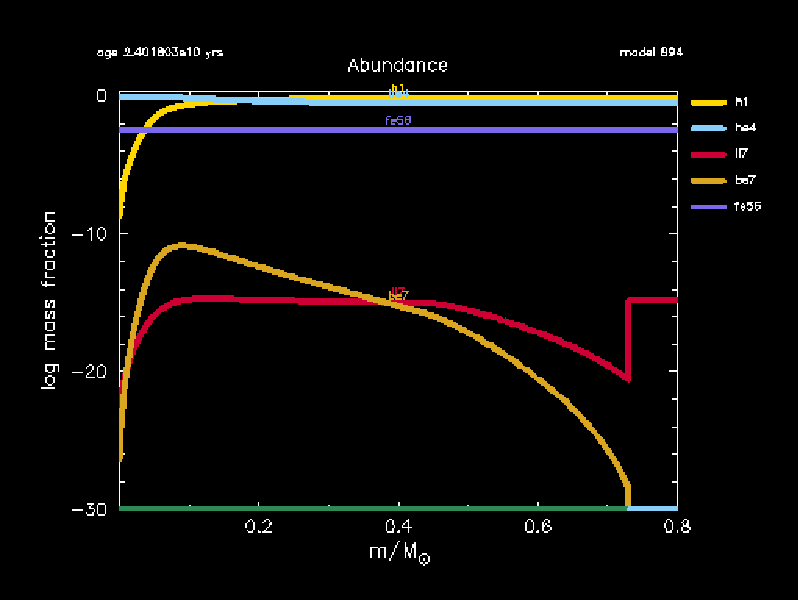
\includegraphics[width=0.5\textwidth]{img/tesis/abundances.pdf}
    \caption {Gráfica de abundancias en la que aparecen los elementos H, He, Fe, Li y Be. El eje de abscisas ha sido reescalado}
    \label{fig:abundances}
\end{figure}

Continuando con el marco físico a simular, pasamos a centrarnos en la activación de los mecanismos que, acorde a la teoría, tienen influencia en el agotamiento del Li:
\begin{itemize}
    \item Proceso de difusión
    \item Proceso de rotación
\end{itemize}

Como ya se indicaba en el apartado \ref{subsec_diffusion}:
\begin{center}
    \begin{minipage}{0.9\linewidth}
        \vspace{5pt}%margen superior de minipage
        {\small
        (MESA) calcula la difusión de partículas y la sedimentación gravitacional resolviendo las ecuaciones de Burger a través del método propuesto por Thoul \cite{Thoul1993}. El módulo de difusión trata los elementos presentes en el modelo estelar como pertenecientes a "clases" definidas por el usuario en términos de rangos de masas atómicas.
        }
        \vspace{5pt}%margen inferior de la minipage
    \end{minipage}
\end{center}

De esta información se desprende que el hecho de que al activar la difusión también activamos la sedimentación gravitacional y, de manera indirecta, el módulo \textit{mlt} encargado de calcular los coeficientes de difusión que entran en juego en proceso de mezclado producido a consecuencia de los movimientos convectivos que se produce en el interior de la estrella.\par

Cabe también mencionar el tratamiento por “clases” que realiza MESA. Los isótopos presentes en nuestra red de reacciones nucleares que tienen un peso atómico similar son tratados de forma conjunta por la rutina de difusión en lo que se refiere a su velocidad de difusión. Ésta queda determinada por el isótopo representativo de la “clase”. La agrupación en clases tiene la ventaja de que las simulaciones se ejecutan de una manera más rápida ya que se ahorran cálculos. Por otra parte, tiene el inconveniente de que los resultados pueden llegar a ser menos exactos. En este trabajo hemos optado por desactivar la agrupación en clases a costa de aumentar los tiempos de simulación.\par

En lo que se refiere a la rotación de las capas superficiales de la estrella, MESA permite especificar una velocidad en km/s, que en nuestro caso ha quedado fijada en 20 km/s al ser un valor similar al que tenemos en el Sol.\par

En el Listado \ref{lst:net_params} mostramos la configuración adicional a añadir al proyecto de MESA para poder simular los conceptos teóricos discutidos hasta este momento.
\begin{lstlisting}[language=Fortran, caption={Parametrización de los procesos relacionados con el Li y de las gráficas de salida.}, label={lst:net_params}]
&star_job
  ! Change default net in order to include 
  !reactions for Li and Be
  change_initial_net = .true.
  new_net_name = 'pp_extras.net'
  ! If enable_adaptive_network is true, 
  ! then at each step, 
  ! the system calculates a new set of isos. 
  ! This can cause significant slowdowns
  enable_adaptive_network = .true.

  ! Activate surface rotation and set velocity
  change_v_flag = .true.
  new_v_flag = .true.
  set_initial_surface_rotation_v = .true.
  new_surface_rotation_v = 20 ! km/sec 

  ! Rotation off until near ZAMS
  change_rotation_flag = .false.
  new_rotation_flag = .true.

&controls
  ! toggle element diffusion
  do_element_diffusion = .true.
  ! If true, don't lump elements into 
  ! classes for diffusion. 
  ! Instead, each isotope in the network 
  ! is treated as its 
  ! own separate class. This can cause 
  ! significant slowdowns 
  ! for large nets, so it is off by default.
  diffusion_use_full_net = .true.
  diffusion_use_cgs_solver = .false.

&pgstar
  ! show HR diagram
  ! this plots the history of L,Teff 
  ! over many timesteps
  HR_win_flag = .true.

  ! configure file output 
  HR_file_flag = .true.
  HR_file_interval = 1


  ! show the abundance profile
  Abundance_win_flag = .true.
  num_abundance_line_labels = 1

  ! set how many elements must be shown
  Abundance_num_isos_to_show = 5
  Abundance_which_isos_to_show(1) = 'li7'
  Abundance_which_isos_to_show(2) = 'be7'
  Abundance_which_isos_to_show(3) = 'h1'
  Abundance_which_isos_to_show(4) = 'he4'
  Abundance_which_isos_to_show(5) = 'fe56'

  ! set the max and min value for the y-axis
  Abundance_log_mass_frac_min = -30
\end{lstlisting}

Llegado este punto, hemos conseguido obtener una configuración de proyecto base que recoge las características esenciales de la estrella a simular en MESA, pone en marcha los procesos físicos relacionados con la evolución del Li y es capaz de informar, tanto a través de los ficheros de salida estándar como de las representaciones gráficas, sobre las abundancias de Li a lo largo de la evolución de la estrella en sus etapas de PMS y MS. Como decimos, esta configuración de proyecto y los valores arrojados por la simulación que lo utiliza, nos servirán para establecer el marco de referencia contra el que comparar los valores obtenidos en las nuevas simulaciones que extienden la funcionalidad de MESA.\par

--CONTINUAR POR AQUÍ --

\subsection{Simulaciones extendiendo el marco teórico estándar de MESA}
Una vez que hemos llegado a un punto en el que tenemos una configuración de proyecto que nos permite obtener las abundancias de Li de forma detallada, y además hemos conseguido activar los procesos de difusión y rotación superficial en nuestro modelo, damos paso a una segunda línea de trabajo consistente en extender el funcionamiento de MESA para incorporar nuestras propias rutinas de extensión al simulador. Las consideraciones previas a tener en cuenta son las siguientes:

--INCLUIR AQUÍ ENUMERACIÓN DE PASOS A GRANDES RASGOS--
\begin{itemize}
    \item Entender el ciclo de control aplicado a los pasos de simulación
    \item Extender la rutina de inicialización para incorporar nuestros parámetros
    \item Extender 
\end{itemize}

El planteamiento teórico no es especialmente difícil, lo complicado del mismo es la parte que afecta a MESA. En concreto, localizar las secciones concretas de código en las que se calcula el valor de la gravedad local que afecta a cada elemento de masa que tiene en cuenta la simulación. A esto hay que sumarle el hecho de que MESA está construido de una forma modular, así que es de esperar que no tengamos una única sección de código en el programa donde se calcule este valor de gravedad, sino que cada módulo que, de algún u otro modo, contribuya a la difusión química de los elementos tiene que ser revisado.\par

Con diferencia, el localizar dónde invocar a nuestra rutina de código es la parte más complicada de todo el presente trabajo. Tenemos que detectar los módulos implicados en la difusión de los elementos, con el riesgo que implica que nos dejemos alguno por identificar, analizar su código fuente en detalle para llegar a entender su funcionamiento y realizar la invocación en el punto exacto a nuestra rutina, para alterar así el valor de gravedad calculado por MESA para un determinado diferencial de masa. Adicionalmente, se hace totalmente necesario el revisar la bibliografía en la que se basa la implementación de las rutinas presentes en cada módulo para dotar de contexto y significado a las líneas de código. De otro modo, es casi imposible extraer el trasfondo científico que se encuentra en ellas codificado.\par

--REVISAR PARA ELIMINAR REFERENCIAS A GRAVEDAD. HACERLO GENÉRICO--

Inicialmente teníamos dos módulos candidatos por los que empezar a estudiar su implementación, el de difusión y el de mlt. Por tener éste último un menor número de líneas de código (aproximadamente unas 1800) y encontrarse la implementación restringida a un solo módulo, empezamos por él. Tras una revisión a fondo del mismo se llegó a generar una versión modificada del mismo que calculaba un nuevo valor de gravedad local relacionado con el elemento de masa diferencial. Este nuevo valor tenía en cuenta tanto la masa del planeta, como su distancia a la estrella.\par

Seguidamente pasamos a analizar el código fuente del módulo de difusión que, como mencionábamos, se basa en la implementación de las ecuaciones propuestas en el trabajo de Thoul, et al. (1994). Ya desde los primeros momentos nos dimos cuenta de que el esfuerzo de localizar dónde deberíamos de invocar a nuestra rutina se iba a complicar. La implementación de este módulo es bastante más laboriosa, larga (más de 3500 líneas) y se encuentra repartida entre varios módulos que, a diferencia de lo que ocurría con el de mlt, algunos de ellos no ofrecían la posibilidad de ser extendidos de una manera cómoda. Además de esto, la implementación que se sigue en MESA acaba generando una matriz de coeficientes de difusión en los que el efecto de la gravedad está representado de manera implícita, es decir, no se calcula un valor de gravedad local asociada a un elemento diferencial de masa en un paso previo, de forma análoga a como ocurre en el módulo de mlt, para finalmente acabar derivando el valor del coeficiente de difusión. En este caso se resuelve el sistema de ecuaciones y la contribución de la gravedad sobre el elemento de masa queda recogida en las soluciones al mismo. A la propia dificultad de entender la implementación del código, se sumaba el hecho de tener que deshacer el cálculo de los coeficientes para poder incluir el efecto de nuestra rutina, y esto era algo que se antojaba harto complicado al no disponerse del conocimiento necesario. Estábamos en un punto muerto.

--REVISAR PARA ELIMINAR REFERENCIAS A GRAVEDAD--

\subsection{Rutina de inicialización para las simulaciones}
EXPLICAR EL CONJUNTO DE PARÁMETROS QUE SE LEEN DEL INLIST, Y SIGNIFICADO. TAMBIÉN LOS FLAGS DE DEPURACIÓN
\begin{lstlisting}[language=Fortran, caption={Rutina de inicialización de las simulacions.}, label={lst:extras_ctrl}]
      subroutine extras_controls(id, ierr)
         integer, intent(in) :: id
         integer, intent(out) :: ierr
         type (star_info), pointer :: s
         ierr = 0
         call star_ptr(id, s, ierr)
         if (ierr /= 0) return
         
         original_diffusion_dt_limit = s% diffusion_dt_limit
         s% other_wind => Reimers_then_Blocker
         ! inject our torque routine
         s% other_torque => other_torque_hook

         !debug flags
         debug_use_other_torque = s% x_logical_ctrl(1)
         debug_reset_other_torque = s% x_logical_ctrl(2)
         debug_get_cz_info = s% x_logical_ctrl(3)
         debug_get_core_info = s% x_logical_ctrl(4)
         debug_new_alpha = s% x_logical_ctrl(7)
         debug_mag_field = s% x_logical_ctrl(8)
         debug_j_dot = s% x_logical_ctrl(9)

         !If true, once the radiative core is developed, report always true
         !in is_radiative_core function
         keep_on_rad_core = s% x_logical_ctrl(6)

         !eps thershold
         eps_threshold = s% x_ctrl(2)

         !disk locking
         disk_lt = s% x_ctrl(3)
         disk_omega = s% x_ctrl(4)

         !Variable MLT alpha
         var_mlt_alpha = s% x_logical_ctrl(10)
      
         ! Once you have set the function pointers you want,
         ! then uncomment this (or set it in your star_job inlist)
         ! to disable the printed warning message,
         ! Uncomment these lines if you wish to use the functions in this file,
         ! otherwise we use a null_ version which does nothing.
         s% extras_startup => extras_startup
         s% extras_start_step => extras_start_step
         s% extras_check_model => extras_check_model         
         s% extras_finish_step => extras_finish_step
         s% extras_after_evolve => extras_after_evolve
         s% how_many_extra_history_columns => how_many_extra_history_columns
         s% data_for_extra_history_columns => data_for_extra_history_columns
         s% how_many_extra_profile_columns => how_many_extra_profile_columns
         s% data_for_extra_profile_columns => data_for_extra_profile_columns  
         
         s% job% warn_run_star_extras =.false.             
      end subroutine extras_controls
\end{lstlisting}

\subsection{Rutina de par de torsión}
EXPLICAR QUE SUSTITUIMOS LA RUTINA POR DEFECTO CON LA NUESTRA
\begin{lstlisting}[language=Fortran, caption={Rutina de par de torsión.}, label={lst:torque_hook}]
      subroutine other_torque_hook(id, ierr)
         use const_def
         integer, intent(in) :: id
         integer, intent(out) :: ierr
         type (star_info), pointer :: s

         ierr = 0
         call star_ptr(id, s, ierr)
         if (ierr /= 0) return


         !If disk locking is actived & the star is younger that disk 
         !locking period &
         !star rotates faster than disk locking rotational velocitiy
         if((disk_lt>0).and.(s%star_age<disk_lt).and.(s%omega(1)>disk_omega)) then
            call other_torque_disk_lock(id, ierr)
         else
            call other_torque_mag_brk(id, ierr)
         endif
         
      end subroutine other_torque_hook
\end{lstlisting}

\subsection{Rutina de frenado magnético}
EXPLICAR QUE LOS DOS TIPOS DE RUTINAS: INTESIDAD FIJA, INTENSIDAD VARIABLE
\begin{lstlisting}[language=Fortran, caption={Rutina de frenado magnético.}, label={lst:torque_mb_hook}]
      ! This routine implements a magnetic braking effect.
      ! It distributes among the zones which conforms the convective shell the
      ! loss of angular momentum
      subroutine other_torque_mag_brk(id, ierr)
         use const_def
         integer, intent(in) :: id
         integer, intent(out) :: ierr
         type (star_info), pointer :: s
         integer :: k
         real(dp) :: B, j_dot, r_st
         type (star_zone_info), target :: sz_info, core_info
         type (star_zone_info), pointer :: sz_info_ptr, core_info_ptr
         real(dp), dimension(:), pointer :: mag_brk_jdot
         integer :: jdot_routine !how to distribute the j_dot
         !controls if jdot distribution must only affect the convective zone
         logical :: only_cz
         !controls if jdot distribution must wait till a radiative core is develop
         logical :: wait_rad_core          
         integer :: activated !signals when the jdot routine is activated
         
         !Pointer to structure which conveys information about the convectice
         !and core zones
         sz_info_ptr => sz_info
         core_info_ptr => core_info

         ierr = 0
         call star_ptr(id, s, ierr)
         if (ierr /= 0) return


         !Reset support structures
         allocate(mag_brk_jdot(s% nz))
         s% extra_jdot(:) = 0
         s% extra_omegadot(:) = 0
         activated = 0
         call reset_x_ctrl(s, idx_low_x_ctrl, idx_high_x_ctrl)
         call reset_core_info(core_info_ptr)
         call reset_convective_info(sz_info_ptr)

         !Wait till radiative core is develop?
         wait_rad_core = s% x_logical_ctrl(5)

         !Loss of angular momentum distribution method
         jdot_routine = s% x_integer_ctrl(1)
         only_cz = .true.
         if (jdot_routine /= 0) then
               only_cz = .false.
         end if

         !Get information about the convective zone
         if (only_cz) then
            !Get information about the outter convective zone
            call get_convective_info(s, sz_info_ptr)
         else
            !Get information about the outter convective zone till star surface
            call get_convective_to_surf_info(s, sz_info_ptr)
         end if

         !Get information about the core
         call get_core_info(s, core_info_ptr)


         !Calculate amount of loss of angular moment
         !Magentic field intensity
         B = s% x_ctrl(1)
         if (B < 0) then
            B = calculate_mag_field_intensity_gb(s)
            j_dot = calculate_jdot_rate_gb(s, B)
         else
            j_dot = calculate_jdot_rate_cantiello(s, B)
         end if
         

         ! The MB routine is activated under the following conditions:
         ! - use_other_torque flag is activated in inlist
         ! AND
         ! - the star is losing mass
         ! AND
         ! - the magnetic field intensitive is bigger than 0.0 (allow to 
         ! execute the routine if use_other_torque=.true.)
         ! AND
         ! (
         !   - a radiative core developed isn't required (configured in inlist)
         !   OR
         !   - a radiative core is required AND this was developed
         !)
         if ((s% use_other_torque) .and. (s% mstar_dot<0.0) .and. (B>0.0) .and. &
            (.not. wait_rad_core .or. (wait_rad_core .and. is_core_rad(s)))) then

            activated = 1

            !Distribute the loss of angular momentum
            call distribute_j_dot(s, j_dot, sz_info_ptr, mag_brk_jdot)

            !It happens that s% extra_jdot is longer than s% nz but mag_brk_jdot
            !is just defined
            !for s% nz elements
            s% extra_jdot(1:s% nz) = mag_brk_jdot
         end if
      end subroutine other_torque_mag_brk
\end{lstlisting}

\subsubsection{Rutina de frenado magnético de intensidad constante}
EXPLICAR QUE SUSTITUIMOS LA RUTINA POR DEFECTO CON LA NUESTRA
\begin{lstlisting}[language=Fortran, caption={Rutina de par de torsión.}, label={lst:jdot_cantiello}]
      real function calculate_jdot_rate_cantiello(s, bf_star) result(new_j_dot)
         use const_def
         type (star_info), pointer, intent(in) :: s
         real(dp), intent(in) :: bf_star

         real(dp) :: r_st, m_st, i_st, alfven_r
         real(dp) :: omega_surf, m_dot, eta_surf, v_inf, v_esc

         !Star data
         r_st = s% r(1)
         m_st = s% m(1)
         omega_surf = s% omega(1)
         !omega_surf = s% omega_avg_surf

         ! escape and infinite velocities
         ! 100000 transform from km/s to cm/s
         v_esc = (618 * ((Rsun/r_st)*(m_st/Msun))**0.5) * 100000
         v_inf = 1.92 * v_esc

         !m_dot = s% star_mdot !This gives the mass loss rate in Mstar/year
         m_dot = s% mstar_dot !This in g/s

         eta_surf = ((r_st * bf_star)**2)/(abs(m_dot) * v_inf)

         !Formula 2.3 Cantiello's MESA assigment
         new_j_dot = two_thirds * m_dot * omega_surf * (r_st**2) * eta_surf
    end function
\end{lstlisting}


\subsection{Rutina de distribución de pérdida de momento angular}
EXPLICAR QUE LOS DOS TIPOS DE RUTINAS: INTESIDAD FIJA, INTENSIDAD VARIABLE
\begin{lstlisting}[language=Fortran, caption={Rutina de distribución de pérdida de momento angular.}, label={lst:dis_jdot}]
      subroutine distribute_j_dot(s, total_j_dot, sz_info, mb_jdot_list)
         type (star_info), pointer, intent(in) :: s
         real(dp), intent(in) :: total_j_dot
         type (star_zone_info), pointer, intent(in) :: sz_info
         real(dp), dimension(:), pointer, intent(out) :: mb_jdot_list
         integer :: k
         real(dp) :: sum_jdot, dm_jdot, dm_bar_jdot, factor

         !By default, no lost of angular moment
         mb_jdot_list(:) = 0.0
      
         do k = sz_info% top_zone, sz_info% bot_zone, 1
            !Here the jdot distribution strategy is defined
            !Simple rule of three distribution loss of angular momentum based on the 
            !angular momentum of the zone vs total angular momentum of the convective zone

            !IMPORTANT: Don't forget to divide by dm(k) in order to get an "specific" jdot
            mb_jdot_list(k) = ((s% dm(k) * s% r(k)**2 * total_j_dot) / &
                  (sz_info% d_mass * sz_info% d_radius**2)) / s% dm(k)

         end do
      end subroutine distribute_j_dot

\end{lstlisting}

\endinput
%--------------------------------------------------------------------
% FIN DEL CAPÍTULO. 
%--------------------------------------------------------------------

